\clearpage
\section{Proximal Policy Optimization (PPO)}
\label{sec:ppo}

\subsection{Challenges of Large Policy Updates}

In deep reinforcement learning, the agent improves by updating its policy after collecting experience from the environment. But there is a tricky problem: if the update is too big, the policy can change so much that it starts making terrible decisions. This is a bit like a student who learns one good trick and then overuses it everywhere, even where it does not apply. The agent's performance can collapse overnight.

\begin{figure}[H]
\centering
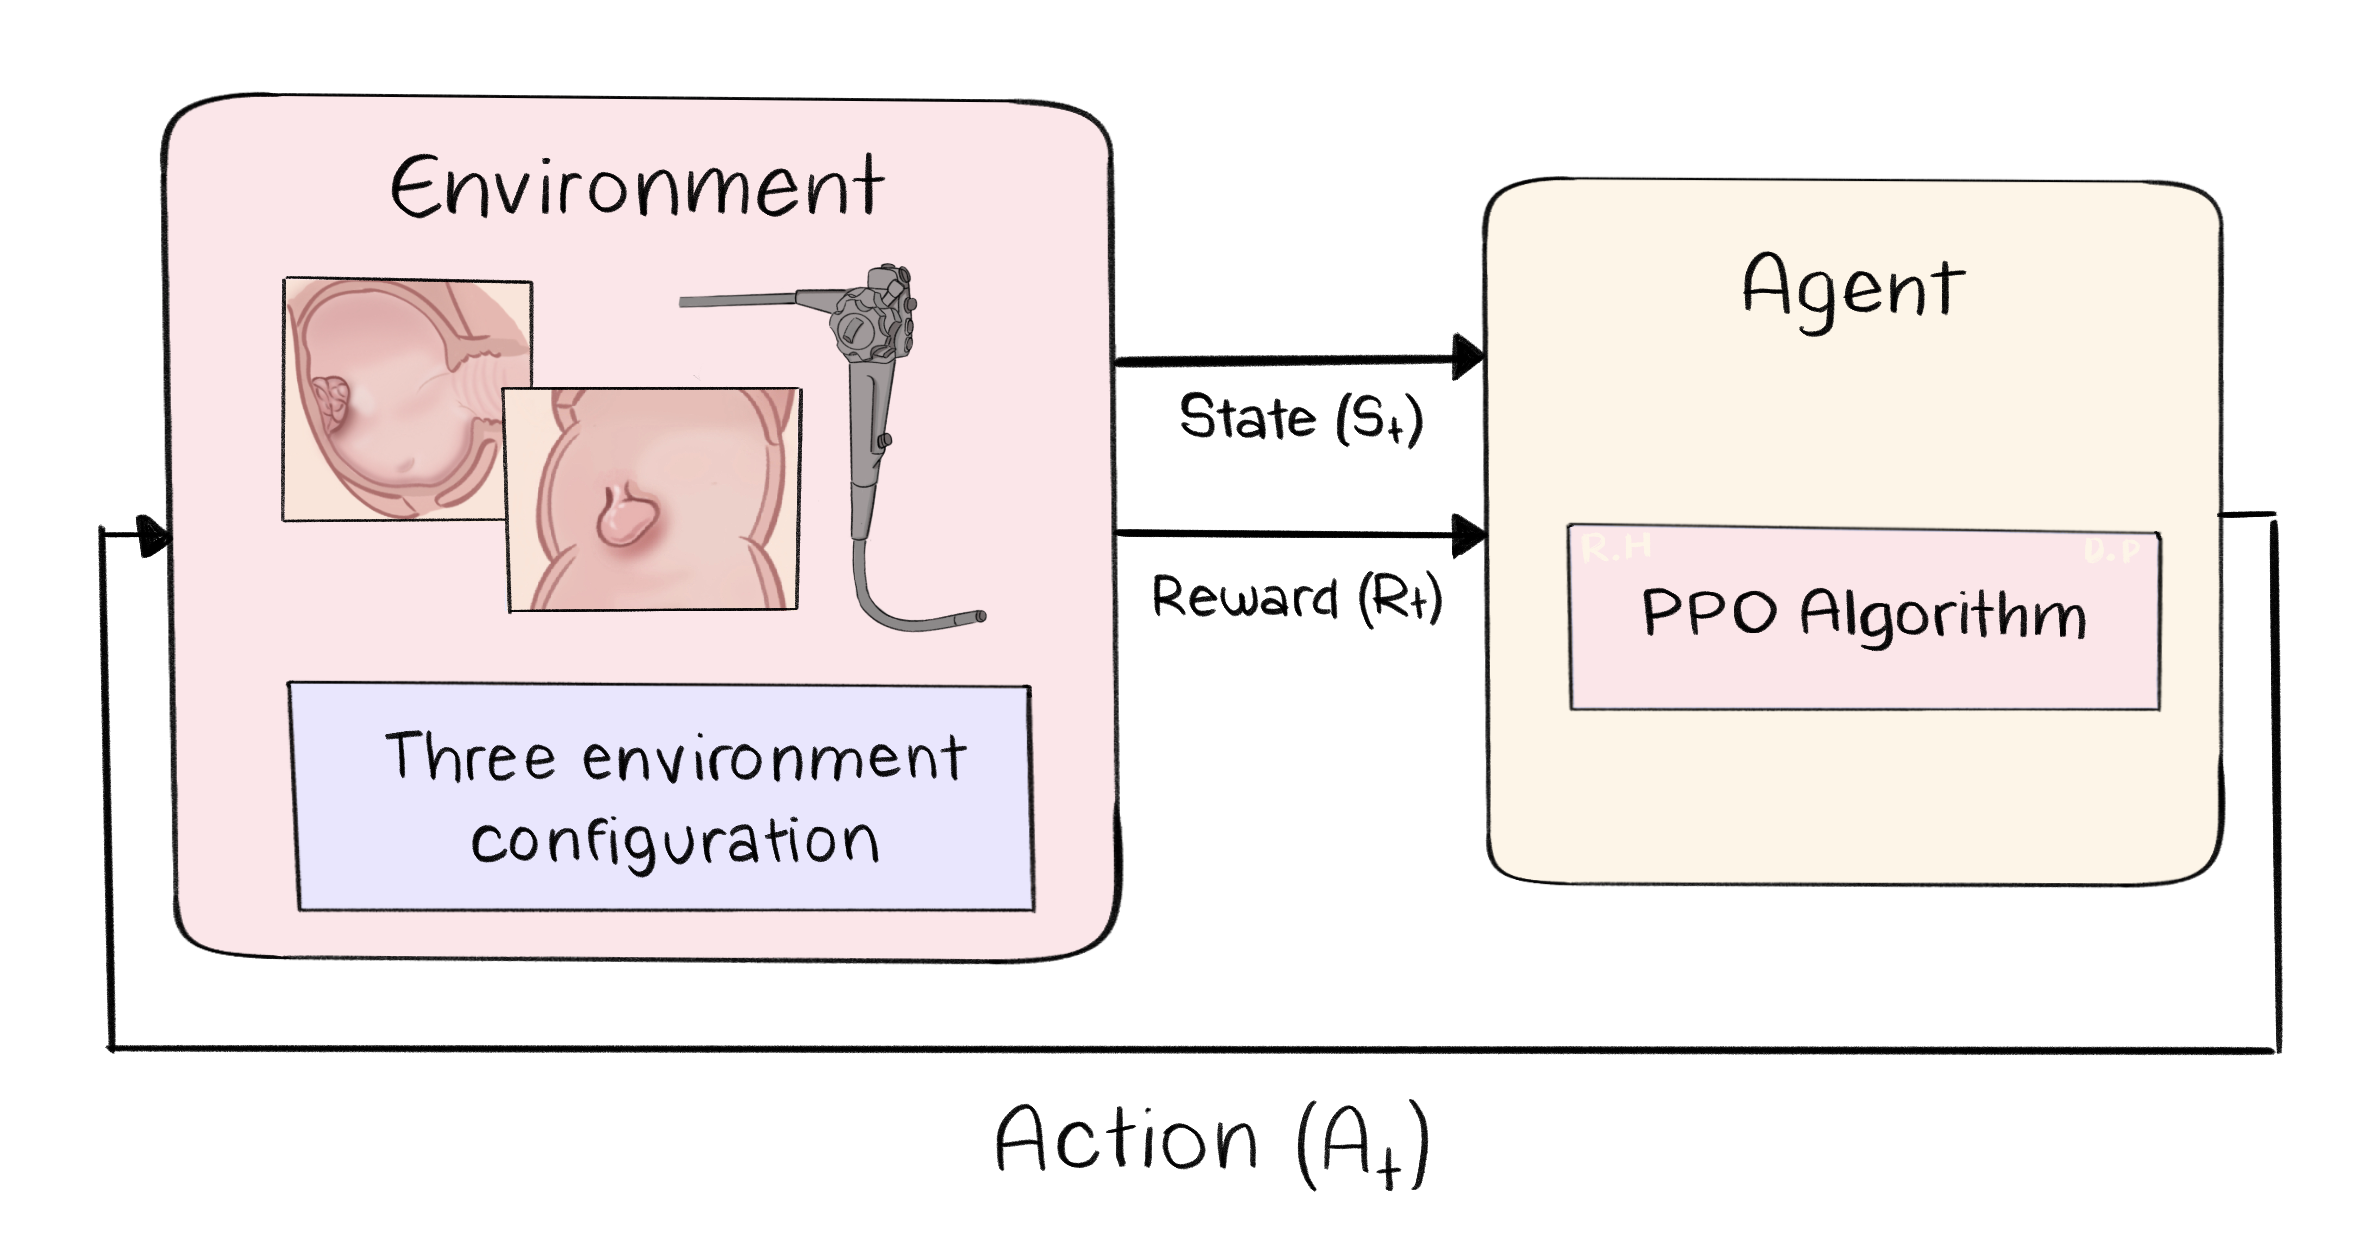
\includegraphics[width=0.8\linewidth]{assets/diagram-ppo-generic.png}
\caption{PPO Generic Architecture}
\label{fig:ppo_generic}
\end{figure}

Early policy gradient methods like \textbf{REINFORCE} suffered from this exact issue \cite{williams1992reinforce}. They had high variance, meaning the learning signal was very noisy, and a single bad update could undo hours of training. To fix this, researchers came up with \textbf{Trust Region Policy Optimization} (TRPO), which adds a mathematical constraint to make sure each update stays small and safe \cite{schulman2015trpo}. The idea is to keep the new policy ``close'' to the old one, measured by a quantity called the \textbf{KL divergence}.

TRPO works well in theory, but it is complicated to implement and slow to run because it needs second-order optimisation (computing the Hessian matrix). That is where PPO comes in.

\subsection{Stabilizing Learning with PPO Clipping}

\textbf{Proximal Policy Optimization} (PPO) was introduced by Schulman et al. at OpenAI in 2017, and it quickly became one of the most popular Deep RL algorithms in the world \cite{schulman2017ppo}. The reason is simple: PPO gives you most of the stability benefits of TRPO, but with a much simpler implementation.

The core idea is to use a \textbf{clipped objective function}. Instead of adding a hard mathematical constraint like TRPO does, PPO clips the policy update so it cannot go too far. Here is how it works:

The algorithm computes a \textbf{probability ratio} $r_t(\theta) = \frac{\pi_\theta(a_t|s_t)}{\pi_{\theta_\text{old}}(a_t|s_t)}$, which tells us how much the new policy differs from the old one for a given action. If this ratio stays close to 1, the update is small. If it gets too far from 1, PPO clips it back. The objective function is:

$$L^{\text{CLIP}}(\theta) = \mathbb{E}\left[\min\left(r_t(\theta) \hat{A}_t,\; \text{clip}(r_t(\theta),\; 1-\epsilon,\; 1+\epsilon)\; \hat{A}_t\right)\right]$$

where $\hat{A}_t$ is the \textbf{advantage estimate} (how much better this action was compared to the average) and $\epsilon$ is the clipping range, usually set to \textbf{0.1 or 0.2}. The $\min$ function makes sure that the agent cannot benefit from making the ratio too large in either direction.

In simple terms: PPO says ``improve, but do not go crazy.'' If the update would change the policy too much, PPO automatically limits it. This is what makes training so stable compared to older methods.


\subsection{The Actor-Critic Setup}

PPO uses an \textbf{actor-critic} architecture, which means it has two components working together:

\begin{itemize}
\item The \textbf{Actor} is the policy network. It takes the current state as input and outputs a probability distribution over possible actions. This is the part that actually decides what to do.
\item The \textbf{Critic} is the value network. It takes the same state as input and outputs a single number: an estimate of how much total reward the agent can expect from this state onwards. This is used to compute the advantage $\hat{A}_t$.
\end{itemize}

The advantage is calculated using \textbf{Generalized Advantage Estimation} (GAE), which combines multiple steps of rewards and value estimates to get a signal that is both low-variance and reasonably accurate \cite{schulman2016gae}:

$$\hat{A}_t = \sum_{l=0}^{T-t-1} (\gamma \lambda)^l \left(r_{t+l} + \gamma V_\phi(s_{t+l+1}) - V_\phi(s_{t+l})\right)$$

In many implementations, including ours, the actor and critic share the same neural network backbone (the CNN and LSTM layers) and only split at the final output heads. This means the visual features learned by the CNN are used by both the policy and the value function, which is more efficient.

The training loop looks like this: the agent collects a batch of experience by interacting with the environment, then uses that batch to update both the actor and the critic over several passes (called \textbf{epochs}). After the update, it throws away the old data and collects a fresh batch. This makes PPO an \textbf{on-policy} algorithm, which means it always learns from data generated by its current policy.

\begin{table}[H]
\centering
\caption{Key PPO hyperparameters and their typical values}
\begin{tabular}{|L{5cm}C{4.5cm}R{5cm}|}
\hline
\textbf{Hyperparameter} & \textbf{Typical range} & \textbf{What it controls} \\ \hline
Clipping range ($\epsilon$) & 0.1 to 0.2 & How much the policy can change per update \\ \hline
Discount factor ($\gamma$) & 0.95 to 0.99 & How much the agent cares about future rewards \\ \hline
GAE lambda ($\lambda$) & 0.9 to 0.99 & Balance between bias and variance \\ \hline
Learning rate & $10^{-4}$ to $10^{-3}$ & Speed of gradient updates \\ \hline
Epochs per update & 3 to 10 & How many passes over each batch \\ \hline
Entropy coefficient & 0.0 to 0.01 & Encourages exploration \\ \hline
\end{tabular}
\label{tab:ppo_hyperparams}
\end{table}

\subsection{Suitability of PPO for the Simulation}

We chose PPO for this project for several practical reasons. First, it is \textbf{stable}. Endoscopy is a task with noisy visual input (reflections, motion blur, changing lighting), and PPO handles that noise well because it does not overreact to any single batch of data. Second, it is \textbf{simple to implement}. The clipped objective is just a few lines of code, and excellent open-source libraries like \textbf{Stable Baselines3} provide ready-to-use PPO implementations. Third, it works well with \textbf{continuous actions}, which is important because our agent needs to output smooth, precise movements rather than choosing from a small set of discrete options.

PPO has also proven itself in many related domains. It is used to train robotic arms in simulation \cite{schulman2017ppo}, to fine-tune large language models with human feedback (the famous RLHF pipeline), and to control agents in complex video games. In surgical robotics, several recent papers have used PPO as their main training algorithm with good results \cite{qian2023arxiv,pore2022iros}.

Finally, PPO pairs well with the rest of our architecture. The CNN extracts visual features, the LSTM adds temporal context, and PPO uses both to learn a policy that improves over time. The clipping mechanism makes sure that even when the simulation produces unexpected situations (a sudden camera movement, an unusual polyp position), the learning process does not break down.

In the Contributions chapter, we will show the exact PPO configuration we used, the reward curves during training, and how the agent's behaviour improved over time.
